\section{Problem 4}

\subsection{Instruction}

Download the gzipped archive \textbf{gridDataUt6.tar.gz} from
http://radionavlab.ae.utexas.edu/datastore/gnssSigProcCourse.
Un-zip and un-tar this file to get access to the underlying files. The
\textbf{*.log} files are columnar-format log files produced by the GRID receiver,
a powerful software-defined radionavigation receiver under development in the UT
Radionavigation Laboratory. The \textbf{*def.txt} files describe the data in the
corresponding \textbf{*.log} files. For now, you’ll only need to pay attention to
\textbf{channel.log}, whose format is described in \textbf{channeldef.txt}.
You’ll find that in this data set there were four L2C-capable GPS satellites
visible over the entire 27-minute data capture interval: those with TXIDs
(PRN identifiers) 7, 8, 19, and 28. For this data set, GRID tracked the signal
type GPS L1 CA on L1 and GPS L2 CL on L2. Draw the file \textbf{channel.log}
(or, equivalently, the file channel.mat) into Matlab and operate on the data to
generate a plot like the one shown in Figure 5.9 in the Misra and Enge textbook
for TXID 7. The plot should include both code- and carrier-derived ionospheric
delay time histories. Generate a second plot showing both the code- and
carrier-derived total electron content (TEC) seen by the signals from the
satellite with TXID 7. Express the value of TEC in TECU. Add a constant offset
to the carrier TEC so that it best matches the code TEC in a least-squares sense.

Answer the following questions:

\begin{itemize}
	\item What could explain the negative values in the final TEC estimates?
	      Is this physically possible?

	\item The ionospheric delay for TXID 7 changes significantly over the 27-minute
	      data capture interval. How is this possible if the GPS satellites move on
	      slow 12-sidereal-hour orbits? (You may wish to inspect the file
	      \textbf{navsol.log} for additional clues.)
\end{itemize}

\textbf{Hints:}\\


\begin{itemize}
	\item Make sure you match pseudorange and carrier phase measurements from the
	      L1 C/A signals with their L2 CL counterparts taken simultaneously.
	\item You’ll want to write a Matlab script to automate the process of drawing
	      in the data and generating the plots for this problem because you’ll
	      need to repeat the procedure in a later problem.
	\item The Matlab files *.mat contain the same data as the corresponding *.log
	      files but in a convenient Matlab format. The following Matlab command
	      sequence (1) draws channel.mat directly into Matlab, (2) stores the
	      contents of the file in the matrix M, (3) finds all the row indices
	      corresponding to the L1 C/A signal of the satellite with TXID 5,
	      (4) loads all the C/N0 measurements from these rows into C\_N0Vec\_txid05:

	      \begin{verbatim}
        >> load channel.mat
        >> M = channel’; // Transpose to get in columnar format
        >> iidum = find(M(:,13) == 0 & M(:,14) == 5);
        >> C_N0Vec_txid05 = M(iidum,9);
        \end{verbatim}
\end{itemize}


\subsection{Solution}

\subsubsection{Main function}

\begin{lstlisting}
  clc; close all; clear all;

  % Load the data
  load("gridDataUt6/channel.mat");
  M = channel';

  % Calculate the Ionopheric delay and plot it
  TXID = 7;
  N_L1 = 5609020;
  N_L2 = 5609020;
  [t, I_L1_code, I_L2_code, I_L1_carrier, I_L2_carrier] = ...
                              dualFreqIonoDelay(M, TXID, N_L1, N_L2);
  fig = plotIonoDelay(t, I_L1_code, 'code', NaN);
  fig = plotIonoDelay(t, I_L1_carrier, 'carrier', fig);
\end{lstlisting}

\subsubsection{Helper function}

\begin{lstlisting}
function [t, I_L1_code, I_L2_code, I_L1_carrier, I_L2_carrier] = ...
                                    dualFreqIonoDelay(M, TXID, N_L1, N_L2)
week2sec = 7 * 24 * 60 * 60;
c = physconst('LightSpeed');
f_L1 = 1575.42 * 1e6;
f_L2 = 1227.60 * 1e6;
lambda_L1 = c / f_L1;
lambda_L2 = c / f_L2;

GPS_L1_CA = 0;
GPS_L2_CL = 2;

% load L1
iidum = find(M(:,13) == GPS_L1_CA & M(:,14) == TXID &...
             M(:,3) ~= 9999 & M(:,10) == 1 & M(:,11) == 0);
ORT_week = M(iidum,3);
ORT_sec_week = M(iidum,4);
ORT_frac_sec = M(iidum,5);
t_L1 = week2sec*ORT_week + ORT_sec_week + ORT_frac_sec;
rho_L1 = M(iidum,8);
phi_L1 = M(iidum,7);

% load L2
iidum = find(M(:,13) == GPS_L2_CL & M(:,14) == TXID  &...
             M(:,3) ~= 9999 & M(:,10) == 1 & M(:,11) == 0);
ORT_week = M(iidum,3);
ORT_sec_week = M(iidum,4);
ORT_frac_sec = M(iidum,5);
t_L2 = week2sec*ORT_week + ORT_sec_week + ORT_frac_sec;
rho_L2 = M(iidum,8);
phi_L2 = M(iidum,7);

% Preprocess (IDK if the L1 and L2 samples coincide temporarly)
t0 = max(t_L1(1), t_L2(1));
tf = min(t_L1(end), t_L2(end));
t = linspace(t0, tf, 1e5);
rho_L1_intrp = spline(t_L1, rho_L1, t);
phi_L1_intrp = spline(t_L1, phi_L1, t);
rho_L2_intrp = spline(t_L2, rho_L2, t);
phi_L2_intrp = spline(t_L2, phi_L2, t);

% Ionospheric delay [Code]
I_L1_code = f_L2^2 / (f_L1^2 - f_L2^2) * (rho_L2_intrp - rho_L1_intrp);
I_L2_code = f_L1^2 / (f_L2^2 - f_L1^2) * (rho_L1_intrp - rho_L2_intrp);

% Ionospheric delay [Carrier]
I_L1_carrier = f_L2^2 / (f_L1^2 - f_L2^2) * ...
       (lambda_L1*(phi_L1_intrp - N_L1) - lambda_L2*(phi_L2_intrp - N_L2));
I_L2_carrier = f_L1^2 / (f_L2^2 - f_L1^2) * ...
       (lambda_L2*(phi_L2_intrp - N_L2) - lambda_L1*(phi_L1_intrp - N_L1));

end
\end{lstlisting}

\subsubsection{Results}

Figure~\ref{fig:ex4_iono_delay} shows the ionospheric delay calculated by
dual-frequency GPS.

\begin{figure}[H]
	\centering
	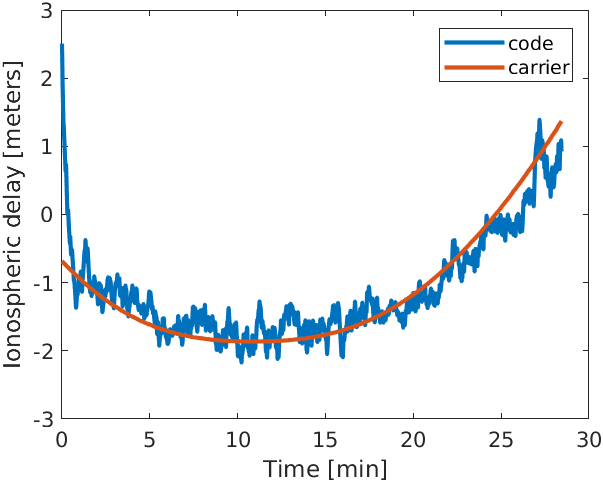
\includegraphics[width=0.9\textwidth]{figs/ex4_iono_delay.png}
	\caption{Ionospheric delay measured using code and carrier dual-frequency GPS.}
	\label{fig:ex4_iono_delay}
\end{figure}

The values shown in Figure~\ref{fig:ex4_iono_delay} are negative. This is not
physically possible. So, the must be related to some delay in the electronics
of the physical transmitter or receiver.

The rapid change in ionospheric delay could be due to the fact that the data
seems to be comming from a receiver in LEO orbit. This can be seen by analyzing
the navsol.log file. The height seem to vary from 100 to 600 km and the
velocity seems to range from 7500 to 8000 m/s. Knowing that Dr. Humphreys has a
receiver in the ISS I wouldn't be surprised if the data would be comming from
there. Thus, the rapid movement of the receiver through the ionosphere explains
the fast fluctuation of ionospheric delay.
